%% ============================================================
%%  Fashion Agent: An LLM-Powered Multimodal Fashion Retrieval
%%  System Based on RAG and ReAct Agent Architecture
%%  Article for LLM Thesis --- English
%%  Compiled with: pdflatex fashion_agent_article.tex
%% ============================================================
\documentclass[12pt,a4paper]{article}

%% ── Encoding & language ──────────────────────────────────────
\usepackage[utf8]{inputenc}
\usepackage[T1]{fontenc}
\usepackage[english]{babel}

%% ── Typography ──────────────────────────────────────────────
\usepackage{lmodern}
\usepackage{microtype}

%% ── Page layout ─────────────────────────────────────────────
\usepackage[left=2.5cm,right=2.5cm,top=2.5cm,bottom=2.5cm]{geometry}
\linespread{1.3}

%% ── Headers / footers ────────────────────────────────────────
\usepackage{fancyhdr}
\pagestyle{fancy}
\fancyhf{}
\fancyhead[L]{\small Fashion Agent: RAG + ReAct Architecture}
\fancyhead[R]{\small LLM Thesis}
\fancyfoot[C]{\thepage}
\renewcommand{\headrulewidth}{0.4pt}

%% ── Math ─────────────────────────────────────────────────────
\usepackage{amsmath,amssymb}

%% ── Graphics & color ─────────────────────────────────────────
\usepackage{graphicx}
\usepackage{xcolor}

%% ── TikZ diagrams ────────────────────────────────────────────
\usepackage{tikz}
\usetikzlibrary{shapes.geometric, shapes.multipart, arrows.meta,
                positioning, fit, backgrounds, calc,
                decorations.pathreplacing}

%% ── Tables ───────────────────────────────────────────────────
\usepackage{booktabs}
\usepackage{tabularx}
\usepackage{multirow}
\usepackage{array}
\usepackage{float}

%% ── Code listings ────────────────────────────────────────────
\usepackage{listings}
\definecolor{codegreen}{rgb}{0,0.55,0.27}
\definecolor{codegray}{rgb}{0.45,0.45,0.45}
\definecolor{codepurple}{rgb}{0.45,0.0,0.65}
\definecolor{backcolour}{rgb}{0.97,0.97,0.97}
\lstdefinestyle{pythonstyle}{
  backgroundcolor=\color{backcolour},
  commentstyle=\color{codegreen}\itshape,
  keywordstyle=\color{blue}\bfseries,
  numberstyle=\tiny\color{codegray},
  stringstyle=\color{codepurple},
  basicstyle=\ttfamily\footnotesize,
  breaklines=true,
  captionpos=b,
  keepspaces=true,
  numbers=left,
  numbersep=5pt,
  showspaces=false,
  showtabs=false,
  tabsize=2,
  language=Python,
  frame=single,
  rulecolor=\color{gray!40},
}
\lstset{style=pythonstyle}

%% ── Caption styling ──────────────────────────────────────────
\usepackage[font=small,labelfont=bf]{caption}
\usepackage{subcaption}

%% ── Hyperlinks ───────────────────────────────────────────────
\usepackage{hyperref}
\hypersetup{
  colorlinks=true,
  linkcolor=blue!60!black,
  citecolor=green!50!black,
  urlcolor=blue!60!black,
  pdftitle={Fashion Agent: LLM-Powered Multimodal Fashion Retrieval},
  pdfauthor={LLM Thesis},
}

%% ── Abstract env ─────────────────────────────────────────────
\usepackage{abstract}
\renewcommand{\abstractnamefont}{\normalfont\bfseries}

%% ── Misc ─────────────────────────────────────────────────────
\usepackage{enumitem}

%% ── Custom colors ────────────────────────────────────────────
\definecolor{agentblue}{RGB}{30,100,200}
\definecolor{agentgreen}{RGB}{34,139,34}
\definecolor{agentorange}{RGB}{220,100,0}
\definecolor{agentred}{RGB}{180,30,30}
\definecolor{agentgray}{RGB}{110,110,110}
\definecolor{lightblue}{RGB}{220,235,255}
\definecolor{lightgreen}{RGB}{220,245,220}
\definecolor{lightorange}{RGB}{255,240,220}
\definecolor{lightred}{RGB}{255,225,225}
\definecolor{lightgray}{RGB}{245,245,245}
\definecolor{darkbg}{RGB}{40,44,52}

%% ============================================================
\begin{document}

%% ── Title block ──────────────────────────────────────────────
\begin{titlepage}
\centering
\vspace*{1.5cm}

{\Large\bfseries\color{agentblue}
  Fashion Agent: An LLM-Powered Multimodal\\[6pt]
  Fashion Retrieval System}\\[0.8cm]

{\large Based on Retrieval-Augmented Generation\\
and ReAct Agent Architecture}\\[1.5cm]

\rule{0.6\textwidth}{1pt}\\[1.5cm]

{\large LLM Thesis --- Technical Report}\\[0.5cm]
{\normalsize University of Information Technology (UIT)\\
Faculty of Computer Science}\\[2cm]

\begin{tabular}{rl}
  \textbf{Author:}   & [Student Name] \\[4pt]
  \textbf{ID:}       & [Student ID] \\[4pt]
  \textbf{Advisor:}  & [Advisor Name] \\[4pt]
  \textbf{Semester:} & [Semester / Academic Year] \\[4pt]
  \textbf{Date:}     & March 2026 \\
\end{tabular}

\vfill
{\small\color{gray}
  \texttt{fashion\_agent\_article.tex} $\cdot$ pdfLaTeX}
\end{titlepage}

%% ── Abstract ─────────────────────────────────────────────────
\begin{abstract}
\noindent
We present \textbf{Fashion Agent}, an intelligent multimodal fashion
retrieval system that combines Retrieval-Augmented Generation (RAG)
with a proactive ReAct (Reason + Act) agent loop.
The system evolves through two phases:
\emph{RAG v1.0}, a fixed nine-step hybrid-search pipeline using
BM25 and Marqo-FashionSigLIP (768-d) vector embeddings; and
\emph{Agent v2.0}, which introduces intent classification,
a clarification gate, session memory backed by PostgreSQL, and
a full ReAct orchestration loop powered by Gemini 2.5 Flash.
A BAAI/BGE cross-encoder reranker and Gemini-driven query expansion
further improve retrieval precision.
End-to-end evaluation targets show Hit Rate@5 $\geq 93\%$,
MRR $\geq 0.80$, and a P95 latency under 15 seconds.
This article details the technical architecture, processing
workflows, and key design decisions behind the system.
\end{abstract}

\tableofcontents
\newpage

%% ============================================================
\section{Introduction}
\label{sec:intro}
%% ============================================================

Fashion e-commerce demands more than simple keyword matching.
Shoppers express intent in colloquial language
(``something smart for a Monday office meeting''),
mix languages, and expect coherent multi-turn conversations.
Classical retrieval systems fail on all three counts.

\textbf{Fashion Agent} addresses these limitations through three
complementary mechanisms:
\begin{enumerate}[label=(\arabic*)]
  \item \textbf{Hybrid retrieval} --- lexical BM25 for exact color/category matching combined with a fashion-specific SigLIP encoder for semantic similarity.
  \item \textbf{LLM-orchestrated reasoning} --- Gemini 2.5 Flash classifies intent, expands queries, asks clarifying questions, and synthesizes a natural-language response, all inside a bounded ReAct loop.
  \item \textbf{Persistent session memory} --- PostgreSQL stores cross-turn context, liked products, and accumulated user preferences.
\end{enumerate}

The system processes \textbf{text-to-image} search (PATH 1):
a natural-language query returns ranked product images with
styling commentary, backed by a dataset of clothing images enriched
with LLM-generated captions and fine-grained color labels.

\subsection{Scope of This Article}

This article focuses exclusively on the \emph{technical architecture
and processing workflows} of Fashion Agent v2.0 (PATH 1).
Section~\ref{sec:data} covers data preprocessing;
Section~\ref{sec:rag} describes the hybrid retrieval core (RAG v1.0);
Section~\ref{sec:agent} details the full agent pipeline;
Section~\ref{sec:eval} presents evaluation metrics;
Section~\ref{sec:deploy} outlines the deployment stack.

%% ============================================================
\section{Data Preprocessing Pipeline}
\label{sec:data}
%% ============================================================

\subsection{Dataset}

Training data originates from the \emph{Clothing Dataset Full}
(Kaggle), a curated set of fashion product images.
Each sample provides: an image identifier, a category label,
and an optional color annotation.
Two preprocessing problems motivate the pipeline:
(1)~noisy labels (\texttt{Not sure}, \texttt{Skip},
\texttt{Other}) that degrade retrieval precision;
(2)~short labels that are too sparse for meaningful semantic embedding.

\subsection{Preprocessing Workflow}

Figure~\ref{fig:preprocess} shows the full pipeline.

\begin{figure}[H]
\centering
%% ── TikZ: Preprocessing Pipeline ───────────────────────────
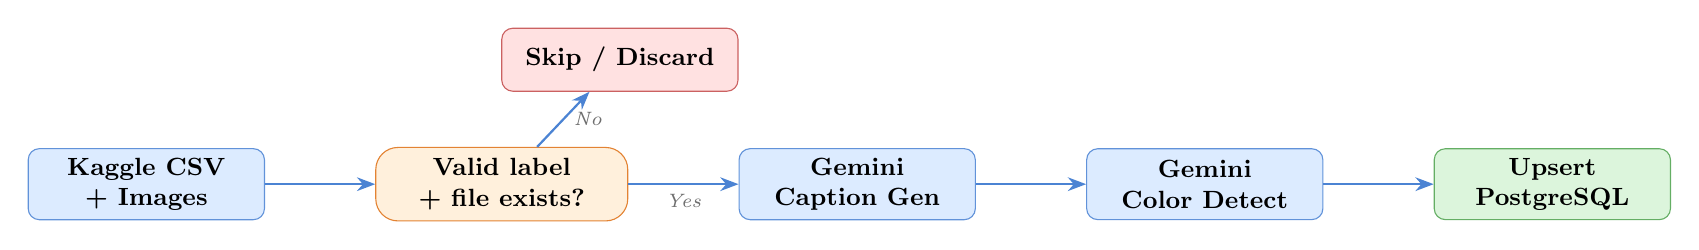
\begin{tikzpicture}[
  node distance=0.55cm and 1.4cm,
  box/.style={
    draw=agentblue!70, fill=lightblue, rounded corners=4pt,
    minimum width=3.0cm, minimum height=0.9cm,
    font=\small\bfseries, align=center
  },
  arrow/.style={-Stealth, thick, color=agentblue!80},
  label/.style={font=\scriptsize\itshape, text=agentgray},
  decision/.style={
    draw=agentorange!80, fill=lightorange,
    rounded corners=8pt,
    minimum width=3.2cm, minimum height=0.85cm,
    font=\small\bfseries, align=center,
    inner sep=4pt
  },
  goodbox/.style={
    draw=agentgreen!70, fill=lightgreen, rounded corners=4pt,
    minimum width=3.0cm, minimum height=0.9cm,
    font=\small\bfseries, align=center
  },
  badbox/.style={
    draw=agentred!70, fill=lightred, rounded corners=4pt,
    minimum width=3.0cm, minimum height=0.8cm,
    font=\small\bfseries, align=center
  },
]

\node[box]  (csv)   {Kaggle CSV\\+ Images};
\node[decision, right=of csv]    (filter) {Valid label\\+ file exists?};
\node[badbox,  above=0.7cm of filter, xshift=1.5cm] (skip) {Skip / Discard};
\node[box,  right=of filter] (gemini)  {Gemini\\Caption Gen};
\node[box,  right=of gemini] (color)   {Gemini\\Color Detect};
\node[goodbox, right=of color] (pg)   {Upsert\\PostgreSQL};

\draw[arrow] (csv)    -- (filter);
\draw[arrow] (filter) -- node[label, below]{Yes} (gemini);
\draw[arrow] (filter) -- node[label, right]{No}  (skip);
\draw[arrow] (gemini) -- (color);
\draw[arrow] (color)  -- (pg);

\end{tikzpicture}
\caption{Data preprocessing pipeline: noisy records are discarded,
         valid items receive LLM-generated captions and color labels,
         then are stored in PostgreSQL.}
\label{fig:preprocess}
\end{figure}

\paragraph{Label filtering.}
Records whose \texttt{label} field belongs to the exclusion set
$\{\texttt{"Not sure"}, \texttt{"Skip"}, \texttt{"Other"}\}$,
or whose image file is missing, are silently skipped.

\paragraph{Caption generation.}
Each product image is passed to \emph{Gemini~2.5 Flash} alongside a
structured prompt that requests a 30\,--\,40-word description
emphasising fabric, silhouette, construction detail, and aesthetic.
Colors and brand names are deliberately excluded to keep the
representation general.
The resulting \emph{caption} acts as a semantic token ---
richer than a bare category label and therefore much more
informative for embedding-based retrieval.

\paragraph{Color labeling.}
A second Gemini call extracts a precise, granular color annotation
(e.g., \textit{``Charcoal Grey''} rather than \textit{``Grey''}).
This field feeds BM25 keyword matching and soft-filter logic.

\paragraph{Batch processing \& checkpointing.}
Items are processed in batches of 20 with
\texttt{asyncio.sleep()} throttling.
PostgreSQL is committed after every batch, providing crash
resilience across the full dataset ingestion run.

\subsection{Schema Design}

\begin{table}[H]
\centering
\begin{tabularx}{\linewidth}{llX}
\toprule
\textbf{Column} & \textbf{Type} & \textbf{Description} \\
\midrule
\texttt{image\_id}  & TEXT   & Unique slug from Kaggle filename \\
\texttt{label}      & TEXT   & Fashion category (T-Shirt, Dress, ...) \\
\texttt{color}      & TEXT   & Fine-grained color from Gemini \\
\texttt{caption}    & TEXT   & 30–40-word LLM-generated description \\
\texttt{image\_path}& TEXT   & Absolute path to JPEG on disk \\
\texttt{created\_at}& TIMESTAMPTZ & Ingestion timestamp \\
\bottomrule
\end{tabularx}
\caption{PostgreSQL \texttt{fashion\_items} schema.}
\end{table}

%% ============================================================
\section{Hybrid Retrieval Core (RAG v1.0)}
\label{sec:rag}
%% ============================================================

\subsection{Overview}

The retrieval backend combines two complementary search paradigms
to maximize both \emph{precision} (exact keyword matching) and
\emph{recall} (semantic similarity):

\begin{itemize}
  \item \textbf{BM25 (lexical)}: Indexes the concatenated string
    \texttt{"\textlangle label\textrangle\ \textlangle color\textrangle"} for each item.
    Excels at exact category/color queries
    (``navy blue shirt'').
  \item \textbf{Marqo-FashionSigLIP (semantic)}: Encodes text queries and images
    into shared 768-dimensional vectors.
    Captures synonyms, style descriptions, and nuanced semantics
    (``relaxed-fit woven cotton pullover'').
\end{itemize}

Results from both retrievers are merged with
\emph{Reciprocal Rank Fusion} (RRF), then re-ranked by a
cross-encoder reranker.

\subsection{Marqo-FashionSigLIP Embedding Model}

\textbf{Why FashionSigLIP over FashionCLIP?}
The \texttt{Marqo/marqo-fashionSigLIP} model produces 768-d vectors
(vs.\ 512-d for FashionCLIP), is fine-tuned on fashion-specific data,
and uses the SigLIP loss (sigmoid-based pairwise rather than softmax),
which generalises better on small downstream domains.
It is served through the \texttt{open\_clip} library, which offers
native Apple MPS (Metal Performance Shaders) support --- important
for development on Apple Silicon hardware.

L\textsubscript{2}-normalised embeddings ensure that dot-product
similarity equals cosine similarity:
\[
  \hat{\mathbf{v}} = \frac{\mathbf{v}}{\|\mathbf{v}\|_2},
  \qquad
  \text{sim}(\hat{\mathbf{u}}, \hat{\mathbf{v}}) =
  \hat{\mathbf{u}} \cdot \hat{\mathbf{v}} \in [-1, 1].
\]

All item captions and labels are embedded offline during indexing
and stored in a \textbf{Qdrant} vector database.
At query time, the user's text is encoded and the $k$-nearest
neighbors are retrieved by approximate nearest-neighbor search.

\subsection{Reciprocal Rank Fusion (RRF)}

RRF avoids the incompatibility of raw BM25 and cosine scores by
blending \emph{rank positions} rather than absolute values:
\[
  \text{score}(d) =
    \frac{w_{\text{bm25}}}{k + r_{\text{bm25}}(d) + 1}
    +
    \frac{w_{\text{vec}}}{k + r_{\text{vec}}(d) + 1}
\]
where $k=60$ acts as a rank smoothing constant,
$w_{\text{bm25}} = 1.0$, and $w_{\text{vec}} = 2.5$.
The higher weight on vector search reflects its superior semantic
coverage.

\subsection{Query Expansion}

Before retrieval, Gemini 2.5 Flash expands the user's query
into a set of synonym sub-queries (e.g., \textit{``red dress''}
$\to$ [``scarlet gown'', ``crimson frock'', ``ruby evening dress'']).
Each sub-query is searched independently;
results are aggregated and re-fused.
This substantially improves recall for terse or colloquial inputs.

\subsection{BGE Cross-Encoder Reranker}

After fusion, the top-$N$ candidates are passed to
\textbf{BAAI/bge-reranker-v2-m3}, a \emph{cross-encoder} model
that jointly encodes the query and each candidate passage
and produces a fine-grained relevance score.
Unlike bi-encoders (which embed query and document independently),
the cross-encoder has access to query-document interactions,
yielding significantly higher precision at the cost of higher latency.
The reranker is applied to the top-20 RRF results, returning the top-5.

\subsection{Retrieval Pipeline Architecture}

\begin{figure}[H]
\centering
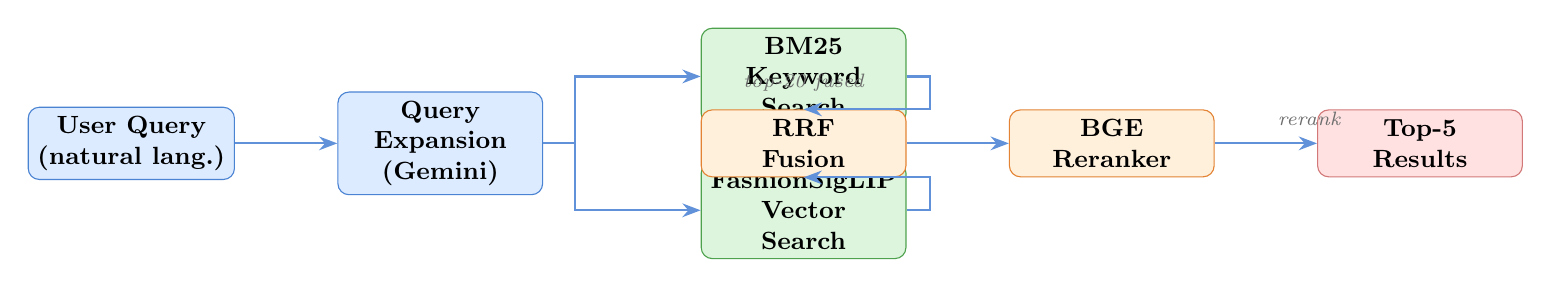
\begin{tikzpicture}[
  node distance=0.5cm and 1.3cm,
  qbox/.style={draw=agentblue!80, fill=lightblue, rounded corners=4pt,
               minimum width=2.6cm, minimum height=0.85cm,
               font=\small\bfseries, text centered, align=center},
  rbox/.style={draw=agentgreen!80, fill=lightgreen, rounded corners=4pt,
               minimum width=2.6cm, minimum height=0.85cm,
               font=\small\bfseries, text centered, align=center},
  obox/.style={draw=agentorange!80, fill=lightorange, rounded corners=4pt,
               minimum width=2.6cm, minimum height=0.85cm,
               font=\small\bfseries, text centered, align=center},
  gbox/.style={draw=agentred!60, fill=lightred, rounded corners=4pt,
               minimum width=2.6cm, minimum height=0.85cm,
               font=\small\bfseries, text centered, align=center},
  arrow/.style={-Stealth, thick, color=agentblue!70},
  label/.style={font=\scriptsize\itshape, color=agentgray},
]

%% Column 0: Input
\node[qbox] (query)  {User Query\\(natural lang.)};

%% Column 1: Expansion
\node[qbox, right=of query] (expand) {Query\\Expansion\\(Gemini)};

%% Column 2: Dual retrieval --- stacked
\node[rbox, right=2.0cm of expand, yshift=0.85cm]  (bm25)   {BM25\\Keyword\\Search};
\node[rbox, right=2.0cm of expand, yshift=-0.85cm] (vec)    {FashionSigLIP\\Vector\\Search};

%% Column 3: Fusion
\node[obox, right=2.0cm of expand] (rrf) {RRF\\Fusion};

%% Column 4: Reranker
\node[obox, right=of rrf]   (rerank) {BGE\\Reranker};

%% Column 5: Output
\node[gbox, right=of rerank] (out)   {Top-5\\Results};

%% Arrows
\draw[arrow] (query)  -- (expand);
\draw[arrow] (expand.east) -- ++(0.4,0) |- (bm25.west);
\draw[arrow] (expand.east) -- ++(0.4,0) |- (vec.west);
\draw[arrow] (bm25.east)   -- ++(0.3,0) |- (rrf.north);
\draw[arrow] (vec.east)    -- ++(0.3,0) |- (rrf.south);
\draw[arrow] (rrf)    -- (rerank);
\draw[arrow] (rerank) -- (out);

%% Labels above arrows
\node[label, above=0.1cm of rrf] {top-20 fused};
\node[label, above=0.1cm of out.west, xshift=-0.1cm] {rerank};

\end{tikzpicture}
\caption{Hybrid retrieval pipeline. The user query is first expanded
         into synonym sub-queries, then searched in parallel via BM25
         and FashionSigLIP vector search. RRF fuses the ranked lists;
         a BGE cross-encoder reranker selects the final top-5.}
\label{fig:retrieval}
\end{figure}

%% ============================================================
\section{Agent v2.0: ReAct Orchestration Pipeline}
\label{sec:agent}
%% ============================================================

\subsection{Architectural Philosophy}

RAG v1.0 executes a fixed nine-step pipeline regardless of query
complexity or available context.
Agent v2.0 replaces this with an \emph{adaptive} Orchestrator +
Sub-agents + ReAct loop model.
Gemini 2.5 Flash acts as the central orchestrator:
it diagnoses intent, decides which tools to invoke, monitors
result quality, and synthesises a natural final response.

The design follows four principles:
\begin{enumerate}[label=(\roman*)]
  \item \textbf{Intent-first} --- classify before acting,
        so downstream modules receive structured, validated signals.
  \item \textbf{Fail fast, clarify early} --- ask for missing
        information rather than guessing and returning poor results.
  \item \textbf{Graceful degradation} --- when results fall below a
        quality threshold, the agent lowers its bar progressively
        and ultimately declines politely.
  \item \textbf{Persistent context} --- session preferences accumulated
        in PostgreSQL influence each new search within the conversation.
\end{enumerate}

\subsection{End-to-End Agent Workflow}

\begin{figure}[H]
\centering
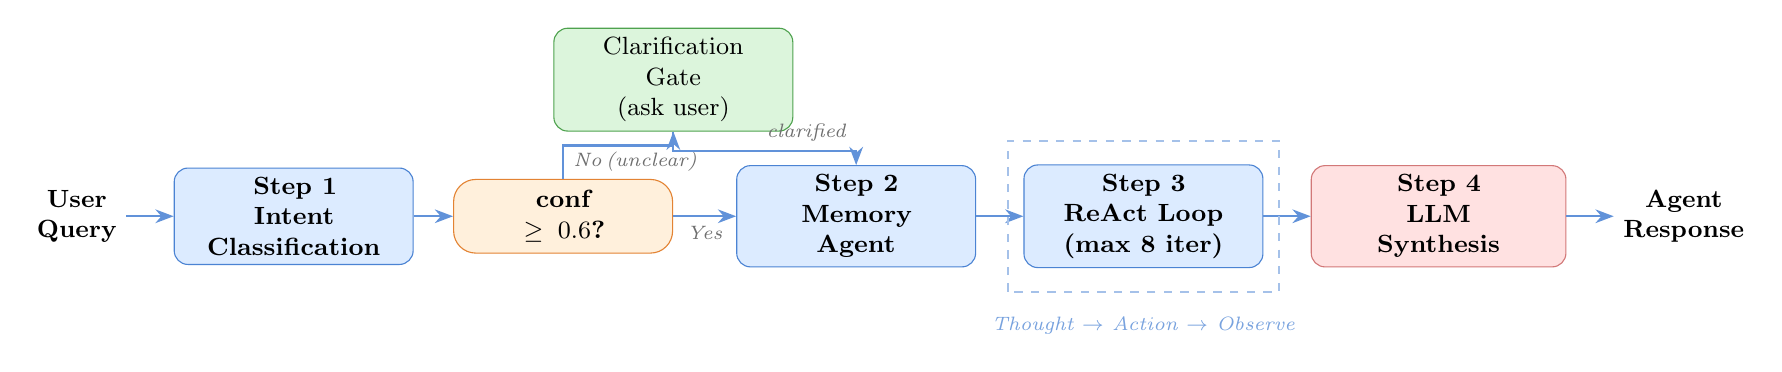
\begin{tikzpicture}[
  node distance=0.55cm and 0.8cm,
  sbox/.style={draw=agentblue!80, fill=lightblue, rounded corners=5pt,
               text width=2.8cm, minimum height=1.0cm,
               font=\small\bfseries, align=center},
  dec/.style={draw=agentorange!80, fill=lightorange,
              rounded corners=8pt,
              text width=2.5cm, minimum height=0.9cm,
              font=\small\bfseries,
              inner sep=4pt, align=center},
  act/.style={draw=agentgreen!80, fill=lightgreen, rounded corners=5pt,
              text width=2.8cm, minimum height=0.9cm,
              font=\small, align=center},
  final/.style={draw=agentred!60, fill=lightred, rounded corners=5pt,
                text width=3.0cm, minimum height=0.9cm,
                font=\small\bfseries, align=center},
  arrow/.style={-Stealth, thick, agentblue!70},
  label/.style={font=\scriptsize\itshape, color=agentgray},
  loop/.style={draw=agentblue!40, thick, dashed},
]

%% Steps (left-to-right across page)
\node[sbox]  (s1)  {\textbf{Step 1}\\Intent\\Classification};
\node[dec,   right=0.5cm of s1]  (d1)  {conf\\$\geq 0.6$?};
\node[act,   above=0.6cm of d1, xshift=1.4cm] (clarify) {Clarification\\Gate\\(ask user)};
\node[sbox,  right=0.8cm of d1]  (s3)  {\textbf{Step 2}\\Memory\\Agent};
\node[sbox,  right=0.6cm of s3]  (s4)  {\textbf{Step 3}\\ReAct Loop\\(max 8 iter)};
\node[final, right=0.6cm of s4]  (s5)  {\textbf{Step 4}\\LLM\\Synthesis};

%% Input / output
\node[left=0.6cm of s1, font=\small\bfseries, align=center] (input) {User\\Query};
\node[right=0.6cm of s5, font=\small\bfseries, align=center] (output) {Agent\\Response};

%% Main flow
\draw[arrow] (input) -- (s1);
\draw[arrow] (s1)    -- (d1);
\draw[arrow] (d1) -- node[label, below]{Yes} (s3);
\draw[arrow] (d1) -- node[label, right]{No\,(unclear)} ++(0,0.9) -| (clarify);
\draw[arrow] (clarify.south) -- ++(0,-0.25) -| node[label, above left]{\scriptsize clarified} (s3.north);
\draw[arrow] (s3) -- (s4);
\draw[arrow] (s4) -- (s5);
\draw[arrow] (s5) -- (output);

%% ReAct sub-loop annotation
\draw[loop] ($(s4.south west)+(-0.2,-0.3)$) rectangle ($(s4.north east)+(0.2,0.3)$);
\node[font=\scriptsize\itshape, color=agentblue!60, below=0.5cm of s4]
  {Thought $\to$ Action $\to$ Observe};

\end{tikzpicture}
\caption{End-to-end Agent v2.0 workflow for PATH~1 (Text-to-Image Search).
         A clarification loop handles ambiguous queries before retrieval.}
\label{fig:agent_flow}
\end{figure}

\subsection{Step 1: Intent Classification}

A few-shot prompt sent to Gemini maps each incoming message to one of
five intent classes (Table~\ref{tab:intents}).
The model also extracts structured \emph{filters}
($\{\texttt{category}, \texttt{color}, \texttt{style},
\texttt{occasion}\}$) and a \emph{refined query} string --- all in
a single LLM call, avoiding a separate slot-filling step.

\begin{table}[H]
\centering
\begin{tabularx}{\linewidth}{llX}
\toprule
\textbf{Intent} & \textbf{Confidence trigger} & \textbf{Agent action} \\
\midrule
\texttt{text\_search}   & $\geq 0.6$        & Execute hybrid search immediately \\
\texttt{outfit\_request}& $\geq 0.6$        & Search + generate outfit advice \\
\texttt{follow\_up}     & any               & Re-use session context, refine search \\
\texttt{out\_of\_scope} & any               & Polite refusal, suggest alternatives \\
\texttt{unclear}        & $< 0.6$           & Invoke clarification gate \\
\bottomrule
\end{tabularx}
\caption{Intent taxonomy and corresponding agent actions.}
\label{tab:intents}
\end{table}

\paragraph{History-aware classification.}
The last four conversation turns are prepended to the prompt.
This allows the classifier to correctly label
\textit{``the white one''} as a \texttt{follow\_up} rather than
\texttt{unclear} when a prior turn established the category context.

\subsection{Step 2: Clarification Gate}

When intent confidence falls below the threshold, the agent invokes
a dedicated clarification module instead of proceeding with a
potentially misspecified search.
A targeted open-ended question is generated by Gemini and returned
to the user.
The user's answer is appended to history, and intent
classification is re-run.

\begin{figure}[H]
\centering
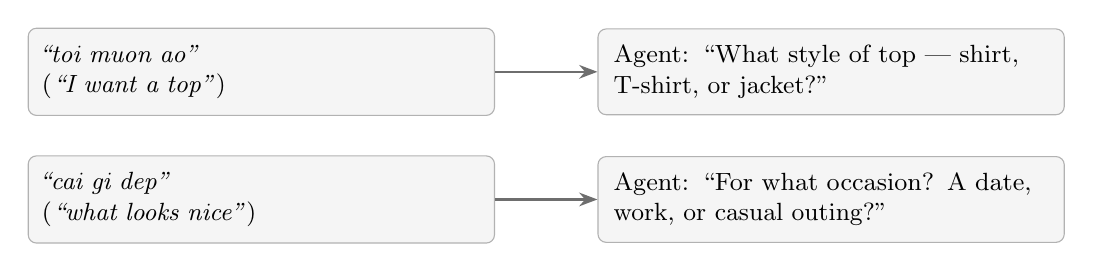
\begin{tikzpicture}[
  node distance=0.45cm and 1.3cm,
  example/.style={draw=gray!60, rounded corners=3pt, fill=gray!8,
                  text width=5.5cm, font=\small, inner sep=6pt},
  arrow/.style={-Stealth, thick, agentgray},
]
\node[example] (q1) {\textit{``toi muon ao''} \\ (\textit{``I want a top''})};
\node[example, right=of q1] (a1) {\small Agent: ``What style of top --- shirt, T-shirt, or jacket?''};
\node[example, below=0.5cm of q1] (q2) {\textit{``cai gi dep''} \\ (\textit{``what looks nice''})};
\node[example, right=of q2] (a2) {\small Agent: ``For what occasion? A date, work, or casual outing?''};
\draw[arrow] (q1) -- (a1);
\draw[arrow] (q2) -- (a2);
\end{tikzpicture}
\caption{Example clarification gate dialogues.
         Vague Vietnamese queries trigger targeted follow-up questions
         in the same language.}
\label{fig:clarify}
\end{figure}

\subsection{Step 3: Memory Agent (PostgreSQL)}

Before executing any retrieval, the agent loads accumulated session
preferences from PostgreSQL.

\begin{itemize}[leftmargin=*]
  \item \textbf{Query history} --- JSONB array of past queries with
        extracted filters (\texttt{color}, \texttt{category}).
  \item \textbf{Liked items} --- JSONB array of products the user
        explicitly approved.
  \item \textbf{Derived preferences} --- the agent counts most-frequent
        colors and categories across history to construct a soft
        preference bias that enriches the search query.
\end{itemize}

\paragraph{Schema highlights.}
Three tables support memory:

\begin{center}
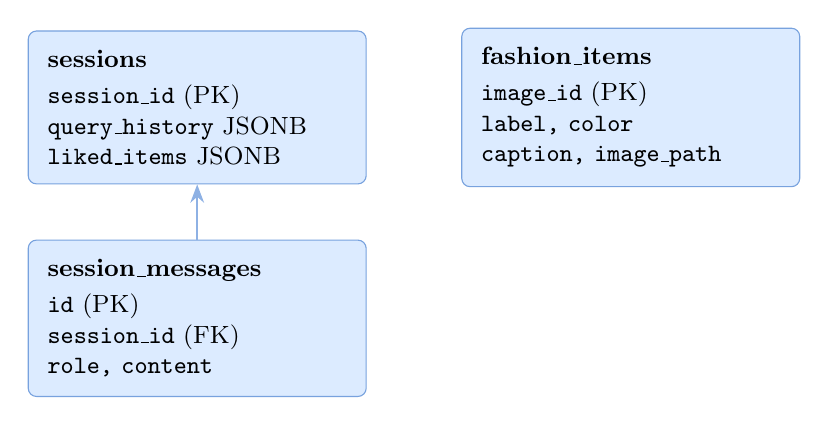
\begin{tikzpicture}[
  tbl/.style={draw=agentblue!60, fill=lightblue, rounded corners=3pt,
              text width=3.8cm, font=\small, inner sep=7pt},
  arrow/.style={-Stealth, thick, agentblue!50},
]
\node[tbl] (sessions) {
  \textbf{sessions}\\[2pt]
  \texttt{session\_id} (PK)\\
  \texttt{query\_history} JSONB\\
  \texttt{liked\_items} JSONB
};
\node[tbl, right=1.2cm of sessions] (items) {
  \textbf{fashion\_items}\\[2pt]
  \texttt{image\_id} (PK)\\
  \texttt{label, color}\\
  \texttt{caption, image\_path}
};
\node[tbl, below=0.7cm of sessions] (msgs) {
  \textbf{session\_messages}\\[2pt]
  \texttt{id} (PK)\\
  \texttt{session\_id} (FK)\\
  \texttt{role, content}
};
\draw[arrow] (msgs.north) -- (sessions.south);
\end{tikzpicture}
\end{center}

\subsection{Step 4: ReAct Loop}

The ReAct loop is the engine of the agent.
At each iteration, the orchestrator takes a
\emph{Thought} (plan which tool to call next),
executes an \emph{Action} (calls up to two tools per iteration),
then inspects the \emph{Observation} (tool output and result quality)
before deciding to continue or stop.

\begin{figure}[H]
\centering
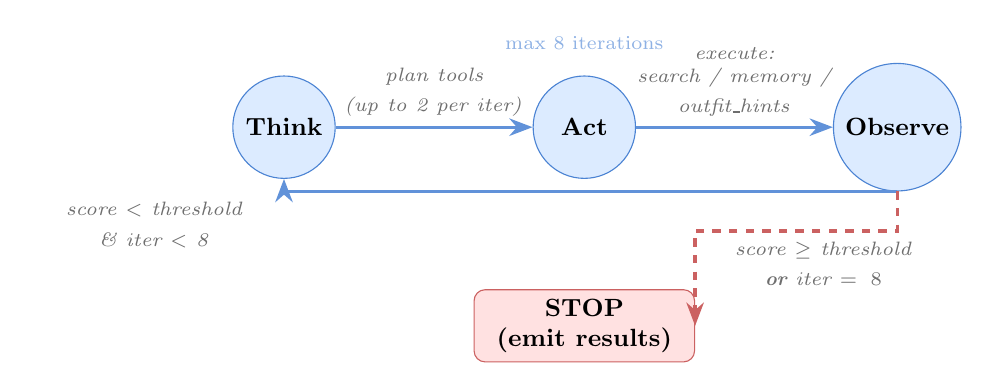
\begin{tikzpicture}[
  node distance=0.8cm and 1.6cm,
  phase/.style={draw=agentblue!80, fill=lightblue, circle,
                minimum size=1.3cm, font=\small\bfseries, text centered},
  arrow/.style={-Stealth, very thick, agentblue!70},
  label/.style={font=\small\itshape, color=agentgray, text width=3cm, align=center},
  stop/.style={draw=agentred!70, fill=lightred, rounded corners=4pt,
               minimum width=2.8cm, minimum height=0.85cm,
               font=\small\bfseries, align=center},
]

\node[phase] (T) {Think};
\node[phase, right=2.5cm of T] (A) {Act};
\node[phase, right=2.5cm of A] (O) {Observe};
\node[stop, below=1.4cm of A] (stop) {STOP\\(emit results)};

%% Circular flow
\draw[arrow] (T.east) -- node[label, above]{\scriptsize plan tools\\(up to 2 per iter)} (A.west);
\draw[arrow] (A.east) -- node[label, above]{\scriptsize execute:\\search / memory /\\outfit\_hints} (O.west);
\draw[arrow] (O.south) -| node[label, below left]{\scriptsize score $<$ threshold\\\& iter $<$ 8} (T.south);
\draw[arrow, agentred!70, dashed] (O.south) -- ++(0,-0.5) -| node[label, below right]{\scriptsize score $\geq$ threshold\\\textbf{or} iter $= 8$} (stop.east);

%% Loop counter
\node[font=\scriptsize, color=agentblue!50, above=0.2cm of A] {max 8 iterations};

\end{tikzpicture}
\caption{ReAct loop structure. Each iteration executes at most two
         tool calls. The loop terminates when retrieved product
         quality passes a dynamic threshold or the iteration cap
         is reached.}
\label{fig:react}
\end{figure}

\paragraph{Dynamic threshold relaxation.}
The loop starts with a score threshold of 0.5.
If no satisfactory result is found within the first four iterations,
the threshold is lowered by 0.2 to allow broader recall.
This two-stage strategy balances precision and coverage.

\paragraph{Available tools.}
\begin{itemize}
  \item \textbf{\texttt{search(query, top\_k)}}: Invokes the full hybrid
    retrieval pipeline (query expansion + BM25 + vector search +
    RRF + reranker).
  \item \textbf{\texttt{memory\_enrich(query, preferences)}}: Rewrites the
    search query by incorporating session-derived color/category
    preferences.
  \item \textbf{\texttt{outfit\_hints(occasion, style)}}: Asks Gemini to
    suggest complementary fashion categories for the given occasion.
\end{itemize}

\subsection{Step 5: LLM Response Synthesis}

Once the ReAct loop completes, all retrieved products,
the full conversation history (last 6 turns), and user preferences
are passed to a final Gemini call that:
\begin{enumerate}[label=(\arabic*)]
  \item selects the most relevant items to mention;
  \item generates a concise 2–4-sentence response
        \emph{in the user's language} (bilingual: English or Vietnamese);
  \item appends a \texttt{styling\_suggestion} for
        \texttt{outfit\_request} queries.
\end{enumerate}

%% ============================================================
\section{Evaluation}
\label{sec:eval}
%% ============================================================

\subsection{Metrics}

\begin{table}[H]
\centering
\begin{tabularx}{\linewidth}{lXcc}
\toprule
\textbf{Metric} & \textbf{Definition} & \textbf{RAG v1.0} & \textbf{Agent v2.0} \\
\midrule
Hit Rate@5  & $\geq 1$ correct item in top-5           & $\geq 90\%$ & $\geq 93\%$ \\
Recall@5    & Fraction of relevant items recalled       & $\geq 85\%$ & $\geq 88\%$ \\
MRR         & Mean Reciprocal Rank of first correct item& $\geq 0.75$ & $\geq 0.80$ \\
Faithfulness& RAGAS --- no hallucinated product info      & ---           & $\geq 0.87$ \\
Task Compl. & Query handled without crash               & ---           & $\geq 95\%$ \\
P95 Latency & End-to-end wall time (95th percentile)   & $<15$\,s    & $<15$\,s   \\
\bottomrule
\end{tabularx}
\caption{Target evaluation metrics comparing RAG\,v1.0 and Agent\,v2.0.}
\label{tab:eval}
\end{table}

\subsection{Comparative Analysis}

\begin{table}[H]
\centering
\begin{tabularx}{\linewidth}{lXX}
\toprule
\textbf{Criterion} & \textbf{RAG v1.0} & \textbf{Agent v2.0} \\
\midrule
Query handling      & Fixed 9-step pipeline          & Adaptive ReAct loop \\
Ambiguous queries   & Search with partial info        & Proactive clarification \\
Multi-turn context  & No memory                       & PostgreSQL session memory \\
Embedding model     & FashionCLIP (512-d)             & FashionSigLIP (768-d) \\
Query expansion     & None                            & Gemini synonym expansion \\
Reranker            & None                            & BGE cross-encoder \\
Response generation & Product list only               & Natural language + styling \\
Storage             & Local CSV files                 & PostgreSQL (server-grade) \\
Out-of-scope detection & None                         & LLM intent gate \\
\bottomrule
\end{tabularx}
\caption{Feature comparison: RAG v1.0 vs.\ Agent v2.0.}
\label{tab:compare}
\end{table}

%% ============================================================
\subsection{Token Usage Measurement}
\label{sec:token}
%% ============================================================

Accurate token tracking is essential for reporting API cost and
understanding the computational budget of each conversation turn.
The system implements \emph{end-to-end token instrumentation}
covering every Gemini call in the pipeline.

%-----------------------------------------
\paragraph{Instrumentation architecture.}

Token counts are extracted directly from the Gemini SDK's
\texttt{response.usage\_metadata} object, which exposes three fields:

\begin{itemize}
  \item \textbf{\texttt{prompt\_token\_count}} --- tokens consumed by
    the input prompt (system message + few-shot examples + user
    context).
  \item \textbf{\texttt{candidates\_token\_count}} --- tokens in the
    model's generated output.
  \item \textbf{\texttt{thoughts\_token\_count}} (Gemini 2.5 Flash) ---
    hidden reasoning tokens used internally during extended thinking;
    currently \emph{not persisted} but available for future capture.
\end{itemize}

Each call is tagged with a \texttt{call\_name} string
(\texttt{"intent"} or \texttt{"synthesis"}) and written
asynchronously to PostgreSQL via \texttt{log\_token\_usage()}.
A database view (\texttt{session\_token\_summary}) aggregates totals
per session on-the-fly:

\begin{verbatim}
CREATE OR REPLACE VIEW session_token_summary AS
SELECT
  s.session_id, s.user_name,
  MAX(u.model_name)                       AS model_name,
  SUM(u.input_tokens)                     AS total_input_tokens,
  SUM(u.output_tokens)                    AS total_output_tokens,
  SUM(u.input_tokens + u.output_tokens)   AS total_tokens,
  s.created_at::date                      AS session_date
FROM llm_token_usage u
JOIN user_sessions s USING (session_id)
GROUP BY s.session_id, s.user_name, s.created_at;
\end{verbatim}

An analytics endpoint (\texttt{GET /analytics/token-usage})
exposes these aggregates to the evaluation dashboard.

%-----------------------------------------
\paragraph{LLM calls per conversation turn.}

Each user message triggers exactly \textbf{two} Gemini API calls
in the happy path, as shown in Table~\ref{tab:token_calls}.

\begin{table}[H]
\centering
\begin{tabularx}{\linewidth}{llXcc}
\toprule
\textbf{Call} & \textbf{Tag} & \textbf{Prompt contents} &
\textbf{Input est.} & \textbf{Output est.} \\
\midrule
Intent classifier &
\texttt{intent} &
System instruction + 5-shot examples + recent history +
user query &
350--600 & 50--120 \\
Response synthesis &
\texttt{synthesis} &
Retrieved products (up to 6) + history (last 6 turns) +
preferences + user query &
1\,500--3\,000 & 200--500 \\
\midrule
\multicolumn{3}{l}{\textbf{Total per turn}} &
1\,850--3\,600 & 250--620 \\
\bottomrule
\end{tabularx}
\caption{Estimated token budget per conversation turn
(Gemini 2.5 Flash, no query expansion, top-6 results).
The intent call is small and fast; synthesis dominates
input cost due to the product context window.}
\label{tab:token_calls}
\end{table}

%-----------------------------------------
\paragraph{Cost estimation.}

Using the Gemini 2.5 Flash pricing schedule
(input \$0.075\,/\,1M tokens; output \$0.30\,/\,1M tokens),
the per-turn API cost is approximately:

\[
C_{\text{turn}} \;=\;
\frac{T_{\text{in}}}{10^6}\times 0.075
\;+\;
\frac{T_{\text{out}}}{10^6}\times 0.30
\;\approx\; \$0.0002 \text{ -- } \$0.0005
\]

At this rate, \textbf{1\,000 conversation turns} cost roughly
\$0.20--\$0.50 in API fees, making the system economically
viable for a thesis-scale evaluation study.

%-----------------------------------------
\paragraph{Analytical query for per-call reporting.}

The following SQL query, run directly against the
\texttt{llm\_token\_usage} table, provides a breakdown
of observed token usage separated by call type:

\begin{verbatim}
SELECT
  call_name,
  COUNT(*)                       AS calls,
  ROUND(AVG(input_tokens))       AS avg_input,
  ROUND(AVG(output_tokens))      AS avg_output,
  SUM(input_tokens+output_tokens)AS total_tokens
FROM llm_token_usage
GROUP BY call_name
ORDER BY total_tokens DESC;
\end{verbatim}

This enables direct comparison of \emph{estimated} budgets
(Table~\ref{tab:token_calls}) against \emph{observed} measurements
from live sessions.

%-----------------------------------------
\paragraph{Known gaps and future work.}

\begin{itemize}
  \item \textbf{Thinking tokens not persisted.}
    Gemini 2.5 Flash allocates an internal reasoning budget
    (\texttt{thoughts\_token\_count}) that is billed separately.
    Capturing this field would give a complete cost picture.
  \item \textbf{Batch synthesis path.}
    The non-streaming \texttt{\_synthesize\_response()} function
    discards \texttt{usage\_metadata}; this is only exercised in
    the batch \texttt{chat()} API and can be patched
    to log on that path as well.
  \item \textbf{Per-call API breakdown not exposed.}
    The analytics endpoint currently aggregates intent + synthesis
    together per session.
    A future version should expose per-\texttt{call\_name} subtotals
    to allow cost attribution to individual pipeline stages.
\end{itemize}

%% ============================================================
\section{Deployment Architecture}
\label{sec:deploy}
%% ============================================================

The production stack is orchestrated with Docker Compose across
four services:

\begin{figure}[H]
\centering
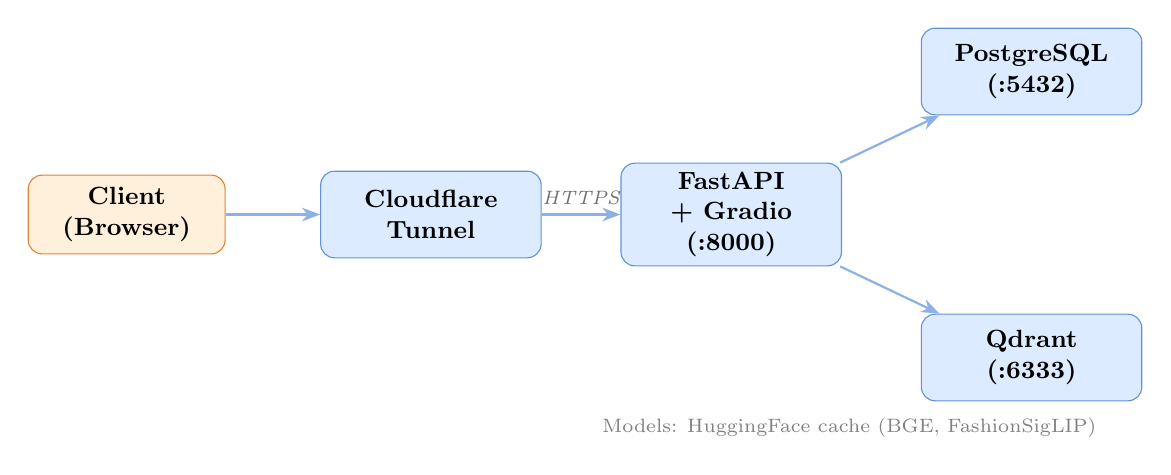
\begin{tikzpicture}[
  node distance=0.7cm and 1.0cm,
  svc/.style={draw=agentblue!70, fill=lightblue, rounded corners=5pt,
              minimum width=2.8cm, minimum height=1.1cm,
              font=\small\bfseries, align=center},
  arrow/.style={-Stealth, thick, agentblue!50},
  label/.style={font=\scriptsize\itshape, color=agentgray},
  client/.style={draw=agentorange!80, fill=lightorange, rounded corners=5pt,
                 minimum width=2.5cm, minimum height=1.0cm,
                 font=\small\bfseries, align=center},
]

\node[client]   (user)    {Client\\(Browser)};
\node[svc, right=1.2cm of user]  (cf)  {Cloudflare\\Tunnel};
\node[svc, right=1.0cm of cf]    (api) {FastAPI\\+ Gradio\\(:8000)};
\node[svc, above right=0.6cm and 1.0cm of api] (pg)   {PostgreSQL\\(:5432)};
\node[svc, below right=0.6cm and 1.0cm of api] (qd)   {Qdrant\\(:6333)};

\draw[arrow] (user) -- (cf);
\draw[arrow] (cf)   -- node[label, above]{HTTPS} (api);
\draw[arrow] (api)  -- (pg);
\draw[arrow] (api)  -- (qd);

\node[font=\scriptsize, color=gray, below=1.8cm of api, xshift=1.5cm]
  {Models: HuggingFace cache (BGE, FashionSigLIP)};

\end{tikzpicture}
\caption{Production Docker Compose deployment.
         Cloudflare Tunnel provides a public HTTPS endpoint without
         exposing ports directly.}
\label{fig:deploy}
\end{figure}

\begin{table}[H]
\centering
\begin{tabular}{llll}
\toprule
\textbf{Service} & \textbf{Image} & \textbf{Port} & \textbf{Role} \\
\midrule
\texttt{postgres}     & \texttt{postgres:16-alpine}     & 5432 & Session memory + item store \\
\texttt{qdrant}       & \texttt{qdrant/qdrant:latest}   & 6333 & Vector similarity search \\
\texttt{fashion-api}  & Custom build (Python~3.11)      & 8000 & FastAPI + Gradio UI \\
\texttt{cloudflared}  & \texttt{cloudflare/cloudflared} & ---    & Secure public tunnel \\
\bottomrule
\end{tabular}
\caption{Docker Compose service inventory.}
\label{tab:docker}
\end{table}

%% ============================================================
\section{Codebase Overview}
\label{sec:codebase}
%% ============================================================

\begin{table}[H]
\centering
\begin{tabular}{llr}
\toprule
\textbf{Module} & \textbf{File} & \textbf{LOC} \\
\midrule
API Layer         & \texttt{api/main.py}                         & 376 \\
Agent Orchestrator& \texttt{agent/fashion\_agent.py}             & 442 \\
Intent Classifier & \texttt{agent/intent\_classifier.py}         & 126 \\
Clarification Gate& \texttt{agent/clarification\_gate.py}        & 110 \\
Session Memory    & \texttt{agent/memory.py}                     & 288 \\
Hybrid Search     & \texttt{search/search\_engine.py}            & 294 \\
Query Expansion   & \texttt{search/query\_expansion.py}          & 106 \\
RRF Fusion        & \texttt{search/fusion.py}                    &  72 \\
BGE Reranker      & \texttt{search/reranker.py}                  & 115 \\
Indexing Pipeline & \texttt{indexing/build\_index.py}            & 470 \\
Data Preprocessing& \texttt{pre\_processing/processing\_data.py} & 698 \\
\midrule
\textbf{Total}    &                                              & \textbf{3{,}097} \\
\bottomrule
\end{tabular}
\caption{Module inventory and lines-of-code breakdown.}
\label{tab:codebase}
\end{table}

%% ============================================================
\section{Key Design Decisions}
\label{sec:design}
%% ============================================================

\begin{enumerate}[leftmargin=*, label=\textbf{D\arabic*.}]

  \item \textbf{768-d FashionSigLIP over 512-d FashionCLIP.}
  The higher-dimensional SigLIP representation captures richer
  fashion semantics and is fine-tuned on the target domain.

  \item \textbf{Caption-as-semantic-token.}
  Rather than embedding bare category labels, each item is indexed
  under a 30–40-word LLM-generated description. This dramatically
  improves recall for descriptive style queries that would otherwise
  never match a short label.

  \item \textbf{BM25 content limited to \texttt{label + color}.}
  Including captions in the BM25 index degrades precision because
  long prose dilutes exact-match signals. Color and category label
  are the only fields where exact keyword matching adds value.

  \item \textbf{RRF over score normalisation.}
  BM25 and cosine similarity are on incompatible scales.
  Score normalisation introduces fragile assumptions; rank-based
  fusion is parameter-light and empirically robust.

  \item \textbf{Cross-encoder reranker at post-fusion stage.}
  Running BGE over all $N$ candidates is too slow; running it only
  over the top-20 RRF results balances latency and precision.

  \item \textbf{PostgreSQL JSONB for session state.}
  Storing query history and liked items as JSONB arrays avoids
  schema migrations as the session data model evolves.
  Atomic JSONB concatenation (\texttt{||}) is race-condition–safe.

  \item \textbf{Bounded ReAct loop with dynamic threshold.}
  A hard cap of 8 iterations prevents runaway latency.
  The two-stage threshold (0.5 $\to$ 0.3 after iteration 4)
  ensures the agent can gracefully escalate recall when precision
  retrieval fails.

\end{enumerate}

%% ============================================================
\section{Risks and Mitigations}
\label{sec:risks}
%% ============================================================

\begin{table}[H]
\centering
\begin{tabularx}{\linewidth}{lXX}
\toprule
\textbf{Risk} & \textbf{Impact} & \textbf{Mitigation} \\
\midrule
High latency (multiple Gemini calls) & ReAct loop adds sequential LLM overhead & Parallel tool calls; cache query expansion results \\
LLM hallucination & Agent fabricates product details & RAGAS faithfulness check; strict JSON output; fallback to product metadata only \\
BM25 rebuild on restart & Cold-start delay & Serialise BM25 index to disk; load at startup \\
PostgreSQL cold start & Connection spikes on container restart & Connection pooling (\texttt{psycopg2} pool); healthcheck service dependency \\
Gemini API rate limit & Batch jobs stall during indexing & Exponential backoff; asyncio throttle (20 items/batch) \\
Dataset label noise & Poor retrieval for edge categories & EXCLUDED\_LABELS filter + LLM caption override \\
\bottomrule
\end{tabularx}
\caption{Risk matrix with mitigations.}
\label{tab:risks}
\end{table}

%% ============================================================
\section{Conclusion and Future Work}
\label{sec:conclusion}
%% ============================================================

Fashion Agent demonstrates that combining a \emph{domain-specific
multimodal embedding model} (Marqo-FashionSigLIP) with an
\emph{LLM orchestration layer} (Gemini 2.5 Flash in a ReAct loop)
yields a retrieval system that is simultaneously more precise
(by leveraging structured intent and session memory) and more
resilient (by clarifying ambiguity rather than guessing), while
maintaining sub-15-second end-to-end latency.

Key contributions of Agent v2.0 over the RAG v1.0 baseline:
\begin{itemize}
  \item Adaptive ReAct loop replacing a rigid 9-step pipeline.
  \item Intent classification eliminating irrelevant searches up front.
  \item Cross-encoder reranker (BGE v2-m3) improving precision without
        sacrificing recall.
  \item Persistent PostgreSQL session memory enabling coherent
        multi-turn dialogue.
  \item Bilingual response synthesis (English/Vietnamese).
\end{itemize}

\paragraph{Future directions.}
\begin{description}
  \item[Phase 3 (Scale)] Expand to 15{,}000–100{,}000 products;
    fine-tune the reranker on fashion-specific relevance labels;
    introduce Redis session caching to reduce PostgreSQL load.
  \item[Phase 4 (Advanced)] Implement virtual try-on
    (IDM-VTON integration); fine-tune FashionSigLIP on proprietary
    inventory; A/B testing of reranker configurations.
  \item[PATH 2 (Image-to-Image)] Allow users to upload a garment photo
    and retrieve visually similar items using composed image search.
\end{description}

%% ── Bibliography placeholder ─────────────────────────────────
\newpage
\begin{thebibliography}{9}

\bibitem{lewis2020rag}
P.~Lewis et~al., ``Retrieval-Augmented Generation for Knowledge-Intensive NLP Tasks,''
\textit{NeurIPS}, 2020.

\bibitem{yao2023react}
S.~Yao et~al., ``ReAct: Synergizing Reasoning and Acting in Language Models,''
\textit{ICLR}, 2023.

\bibitem{bm25}
S.~Robertson and H.~Zaragoza, ``The Probabilistic Relevance Framework: BM25 and Beyond,''
\textit{Foundations and Trends in Information Retrieval}, 2009.

\bibitem{siglip}
Z.~Zhai et~al., ``Sigmoid Loss for Language Image Pre-Training,''
\textit{ICCV}, 2023.

\bibitem{bge_reranker}
S.~Xiao et~al., ``C-Pack: Packaged Resources to Advance General Chinese Embedding,''
\textit{arXiv:2309.07597}, 2023.

\bibitem{rrf}
G.~V.~Cormack, C.~L.~A.~Clarke, and S.~Buettcher,
``Reciprocal Rank Fusion Outperforms Condorcet and Individual Rank Learning Methods,''
\textit{SIGIR}, 2009.

\bibitem{gemini}
Google DeepMind, ``Gemini: A Family of Highly Capable Multimodal Models,''
\textit{arXiv:2312.11805}, 2023.

\end{thebibliography}

\end{document}
